% \chapter{Problem Formulation}
% \label{chap:ProblemFormulation}

% The previous chapter described the literature that contributed towards the support of Proxying Quic streams within kubernetes cluster. It summarized the drawbacks of several different approaches and clearly identified the limitations for the approaches by defininig the gaps of the those approaches. Clearly there is a need to be able to have a solution that enables proxying QUIC streams into kubernetes. In other words, there exists a requirement to distribute and loadbalance http3 multiplexed streams within kubernetes. This chapter focuses on correctly identifying the challenges and clearly stating out the gaps occuring in the traditional proxy servers with regards to supporting webtransport streams. This chapter then proceeds to provide a primary approach for this dissertation in order to realise our end result. This chapter starts by giving an abstracted view of the approach that would solve the problem and arrive at a working solution. The next section talks about the novelty of the proposed approach and how it is different from existing working directions. The section covers the idea on the on the intuition behind chosing the approach following which the targets to be achieved for the stated problem are stated. Finally, the identified challenges are listed for the proposed approach.

% \section{Abstracted View of the solution}
% The main objective of this study is to enable Webtransport independent multiplexed streams to be proxied to different microservices in kubernetes envirnoment. This study aims to provide a complete discrete solution to the problem and solving the core problem which other studies did not solve. In order to arrive at a working solution at a highly abstracted way is to find a way to create a kuberentes supported http3 streams based proxy server.

% \begin{table}[H]
% \centering
% \caption{Abstracted View of Proposed Solution}
% \begin{tabular}{|p{4cm}|p{5.5cm}|p{5.5cm}|}
% \hline
% \textbf{Capability Area} & \textbf{Existing Approaches} & \textbf{Our Approach (Custom Proxy Server)} \\
% \hline
% Stream Visibility & Operate at packet level with no awareness of streams & Enable deep stream-level visibility and context recognition \\
% \hline
% Stream Handling & Entire connection treated as a monolithic flow & Demultiplex and manage streams individually \\
% \hline
% Application-Layer Intelligence & Minimal application-layer insight or control & Enable content-based routing, security, and monitoring per stream \\
% \hline
% \end{tabular}
% \end{table}


% \section{Differences from existing approaches}
% As stated in the previous chapter most of the existing approaches do not address the problem at hand which is independent stream level inspection and control. Most of the approaches use custom annotations in ingress or use third party libraries but finally ends up routing entire UDP packet when it comes to http3 streams to the server. On the other hand work for this specific problem is currently in progress and is being addressed but there has not yet been a working solution which addresses the core problem. Thus, our apporach differs in a way that modification are done to the working quic library implementation to make a progress towards creating a standardized solution. The difference in approaches is shown in the table below





% This section should present a short review of the topics discussed in the State of the Art chapter in order to then discuss gaps in the existing work and the relationship of these gaps to the work described in this dissertation.

% \section{Proposed Work}
% % This section should provide a thorough description of the problem and an overview of the
% % work proposed to address the problem.
% To cater to the problem of Head of the line blocking with TCP, Quic Protocol was incepted and formalized. With Quic streams we are able to leverage the performance benefit only if one can use it at scale. Kubernetes is the state of the art modern solution for deploying applications in containers across multiple machines as microservices and there exists gaps witth regard to the support of quic streams hindering being able to leverage the capability of http3 webtransport streams.  Current solutions in kubernetes does not act as stream forwards but rather act as UDP packet forwarders as they operate at a lower level abstraction rather than providing granular application level visibility. Kubernetes environment is largely based on TCP and Http 1.1 Protocols and support for Http3 streams is not natively support by any Kubernetes objects. The approach to the the solution is addressing the gaps individually. To first address the lack of support by native kuberentes objects the proposed solution would be expected to be deployed as a Pod exposed via service in kubernetes. To address the solution, a custom proxy server supporting acceptance of webtransport streams is proposed. To demonstrate the working prototype a streaming usecase is used along with widely used streaming tools. This approach addresses the problem at hand and provides a suitable working solution/


% Defining the chapter
\chapter{Problem Formulation}

In this chapter, the research problem of this dissertation is determined as the problem of combining modern WebTransport over QUIC protocol \cite{rfc9000} with Kubernetes \cite{kubernetes-docs}. WebTransport \cite{webtransport-draft}, QUIC, Kubernetes are very sophisticated technologies, and integrating the 3 technologies to provide real-time and low latency applications is challenging. This chapter addresses the research gaps based on the State of the Art with additional aspects of it and proposes a new solution to these problems and a clear plan to solve. It also discusses the difference between the proposed methodology and the current methods and provides certain design and implementation objectives in order to obtain a sustainable, production-ready streaming framework.

This chapter effectively explains the problem it wants to address, offers an abstracted solution, tells how the work is different among other solutions and provides a blueprint on how the designed solutions could be attained.

% Section 3.1: Identified Challenges
\section{Identified Challenges}
The State of the Art review highlights that there is substantial advancement in modern transport protocols, cloud-based networking as well as streaming platforms. But it also highlights the issues that act against formation of high-performance and real-time systems in kubernetes. The need to conduct this research is motivated by the following challenges, some of which are briefly explained below.

\subsection{Limited Support for QUIC and HTTP/3 in Kubernetes Ingress Controllers}
Experimental QUIC and HTTP/3 support have been added to Kubernetes Ingress Controllers such as NGINX, HAProxy, and Envoy via controller specific annotations such as \texttt{nginx.org/quic: "true"} (Section 2.6.9.4). Nevertheless, such implementations are unreliable and not production ready. Nginx Controller currently does not support proxying and HAProxy fails to proxy streams. The Gateway Application Programming Interface (API) has a more open model, and allows protocols that use UDP such as QUIC (Section 2.6.10.3), and its utility relies on the capabilities of underlying reverse proxies.

Moreover, proxies like Angie and HAProxy along with the ingress controller cannot inspect or manage individual QUIC streams (Sections 2.6.12, 2.6.13, 2.6.14). This limitation prevents features like stream-aware routing, prioritization, etc which are essential for low-latency applications such as real-time streaming or telemetry. As a result, building efficient, stream-aware systems in Kubernetes remains a challenge.

\subsection{Challenges in Load Balancing for QUIC-Based Traffic}
Unlike the traditional TCP-based protocols, QUIC uses UDP, so it becomes a challenge in Kubernetes environments where the traffic is heavily built on TCP traffic. The cloud service providers, such as Google Cloud, has already implemented support of QUIC in their load balancers with protocol downgrade, whereas on-premise load balancer implementations, such as MetalLB, do not have advanced features such as supporting stream-level routing, autoscaling, or failover (Section 2.6.15.4). MetalLB doesnt support quic proxying and treats HTTP as UDP packets. This creates a challenge in managing QUIC-based traffic in a cluster, which is on-prem, local or privately owned, thus encapsulating the scalability of HTTP/3 applications.


\subsection{Operational Complexity and Observability}

QUIC’s encrypted headers and multiplexed streams in QUIC improve performance and security at the expense of making traffic inspection difficult. Kubernetes environment being largely based on tcp have weak weak support for QUIC, which makes it harder to debug and analyze performance (Section 2.6.10.6). Even the Gateway API decouples infrastructure and application considerations, a misconfiguration of work makes whole operation within kubernetes more difficult (Section 2.6.10.6). These issues create barriers to building reliable, real-time webtransport stream demultiplexers/Routers in kubernetes.

% Section 3.2: Abstracted View of the Solution
\section{Abstracted View of the Solution}


The aim of this dissertation is to open a possibility of allowing independent WebTransport streams to be load balanced to various microservices that run on Kubernetes and  address the critical gap in stream-level inspection, routing, and observability. The recommended solution is the use of a custom HTTP/3/QUIC proxy server that is natively integrated with the cluster and multiplexed streams to internal services, based on content or metadata. WebTransport will have each stream as a separate a logical channel which can send its own data multiplexed over a single connection.


Table 3.1 compares the proposed solution with existing approaches, highlighting the unique capabilities.

\begin{table}[h]
\centering
\caption{Abstracted View of Proposed Solution}
\begin{tabular}{|p{4cm}|p{5cm}|p{5cm}|}
\hline
\textbf{Capability Area} & \textbf{Existing Approaches} & \textbf{Our Approach (Custom Proxy Server)} \\
\hline
Stream Visibility & Operate at packet level, no stream awareness & Enable deep stream-level visibility and context recognition \\
\hline
Stream Handling & Treat entire connection as a monolithic flow & Demultiplex and manage streams individually \\
\hline
Application-Layer Intelligence & Minimal insight or control at application layer & Enable content-based routing, security, and monitoring per stream \\
\hline
\end{tabular}
\end{table}

% Section 3.3: Differences from Existing Approaches
\section{Existing Approaches}
Current solutions, such as those using Angie, HAProxy, or traditional Ingress Controllers, route entire QUIC connections to a single backend without inspecting individual streams. Even when HTTP/3 is supported, these systems lack the ability to manage streams independently, limiting their flexibility for advanced use cases. Annotations and third-party plugins provide partial workarounds, but they are often unstable and controller-specific (Section 2.6.9.4).

This problem is solved in the current technologies with Angie, HAProxy, or legacy Ingress Controllers with custom annotations, where the entire full QUIC connection is sent to the same backend without looking at individual streams. These systems can not manage streams independently thus failing to give flexibility to be used in more advanced use cases even when the underlying protocol such as HTTP/3 supports it. Even using workarounds] with annotations and third-party plugins for ingress, which are unstable and controller-specific they still are limitted to forwarding entire Quic connections (Section 2.6.9.4).

In contrast, this dissertation proposes a novel approach by modifying a production-grade QUIC library, such as Aioquic, to expose and manage HTTP/3 streams. The custom proxy server will:

\begin{itemize}
    \item Inspect stream metadata or payloads to enable content-based routing.
    \item Forward streams independently to different Kubernetes microservices.
    \item Ensure compatibility with WebTransport clients and Kubernetes services.
    \item Provide a standardized, production-ready framework which can be deployed easily across kubernetes clusters.
\end{itemize}
This approach fundamentally differs from existing systems as it prioritizes stream-level granular control which no solution provides while offering flexibility and scalability.

% Section 3.4: Targets
\subsection*{3.4 Targets}
This section outlines the design and implementation goals for the proposed solution, providing a clear roadmap for achieving the dissertation’s objectives.

\subsubsection*{Design Goals}
\begin{itemize}
    \item \textbf{WebTransport Client for Multiplexed Streaming}: Design a WebTransport client that multiplexes audio, video, and chat streams over QUIC to demonstrate real-time, low-latency streaming.
    \item \textbf{Standardized Stream Header Format}: Implement a 32-byte header format to standardize stream identification, length, and type, enabling efficient routing.
    \item \textbf{Single-Node Minikube Cluster}: Use a single-node Minikube cluster with the Docker driver for lightweight, local Kubernetes deployment.
    \item \textbf{Configuration-Driven Components}: Ensure all components support configuration-driven decisions for flexibility and maintainability.
    \item \textbf{HTTP/3 WebTransport Connections}: Establish secure, concurrent HTTP/3 WebTransport connections via MetalLB UDP ingress.
    \item \textbf{Stream-Aware Router}: Build a router that parses stream headers, handles fragmentation, and routes packets based on stream type.
    \item \textbf{Dedicated Microservices for Pulsar Integration}: Create microservices that process data and publish to Apache Pulsar for real-time analytics.
    \item \textbf{Modular Streaming Platform}: Architect a modular, WebTransport-based streaming platform using Kubernetes, Pulsar, and custom proxies.
\end{itemize}

\subsubsection*{Implementation Goals}
\begin{itemize}
    \item \textbf{Comprehensive Installation and Configuration}: Provide detailed guidance on installing and configuring the solution, including Kubernetes, Pulsar, and the custom proxy.
    \item \textbf{Multiplexed Client Streams}: Develop client-side logic to create and manage live, multiplexed streams, such as audio, video, chat.
    \item \textbf{End-to-End Stream Demultiplexing and Routing}: Build software to demultiplex streams and route them to appropriate microservices based on header metadata.
    \item \textbf{YAML-Driven Configurations}: Enable YAML-driven ConfigMaps and Secrets for hot-reloadable, declarative routing and service configurations.
    \item \textbf{Protocol Translation and Analysis}: Use Wireshark to analyze and validate QUIC and HTTP/3 traffic, ensuring correct protocol translation and performance.
\end{itemize}




\section{Summary}
This dissertation addresses the problem of a lack of solutions to understand Http3 streams within Kubernetes, so that a custom solution creating an HTTP3 server that understands HTTP3 streams can be created to proxy it to other Kubernetes services. This dissertation analyses different ways to achieve the targeted result and proposes a solution "Custom H3 Ingress Server" wherein kubernetes' native objects are leveraged in conjuction with Aioquics quic implementation.


\chapter{Design}
\label{chap:Design}

% At the beginning of each chapter, a description should introduce the reader to the content of the chapter. For the Design chapter, this desription should explain to the sections of the chapter, how these sections will explain the overall design and specific details, and the contribution of the individual sections towards the overall chapter.

% The Design chapter should provide a description of the approach that addresses the problem identified above. The intention of this chapter is to discuss a proposed solution at an abstract, high level that is disconnected from an actual realisation of a solution. The motivation for this approach is that it should be possible to implement the proposed solution using a variety of methods; however, the abstract description of the solution should be applicable to a variety of possible realisation. For example, a solution for an issue may have been realised in as a Pascal or C program in the mid-1990s, whereas in the mid-2020s, the same issue may be addressed with a Python or Rust program. 


This chapter outlines the major design decisions taken in this dissertation. The general problem is decomposed into smaller subproblems and each of them is solved one at a time. For every subproblem, the reasoning behind the chosen solution is explained and described using diagrams to understand the flow of communication. Once each part is solved, the solutions are combined to form the final system design

The values taken by major parameters are also described here along with explanation. In the beginning of the chapter, it starts with the design of the WebTransport client, decision made in the process of its development. It then proceeds to explain the architecture of the Kubernetes-based infrastructure upon which the system will be deployed. Then it turns to the essence of the dissertation, namely the WebTransport router and gives detailed design for the same. Subsequently, the chapter will deal with the integration of microservices and Apache Pulsar and the design of this connection. At last, it gives the whole architecture of the system and concludes with a brief conclusion.



\section{Design of Client}
Webtransport Streams were the point of intererst so the first task was to designa  specific usecase for our proplem. The usecase of Webtreaming was considered as it would perfectly fit with our problem. From the gaps in k8s existing solutions,it was evident that a client would be required that sends multiplexed data streams to the kuberenetes cluster. For the streaming usecase in javascript client, Webtransport API supports multiplexing streams of data to be sent over a single connection. So there was a need to design the packet structure as to how the packet would be received at the destination end. 

\subsection{Webtransport Streams}
Webtransport streams operates atop of Quic protocol which helps achieve enabling multiple concurrent unidirectional data streams to be sent within a single secure transport connection. It implied need for multiple dedicated streams. To fit our streaming usecase we have decided audio,video and chat datastreams. These act as seperate datastreams which would indicidually send with isolation. This circumvents the HOL problem. The following table shows the design for multiple streams to be multiplexed and sent over a single connection.


\begin{table}[h!]
\renewcommand{\arraystretch}{0.9}
\small
\centering
\begin{tabularx}{\textwidth}{|l|X|l|l|l|X|}
\hline
\textbf{Stream Name} & \textbf{Purpose} & \textbf{Direction} & \textbf{Reliability} & \textbf{Latency} & \textbf{Notes} \\
\hline
Audio Stream & Transmit PCM audio data & Unidirectional & Medium & High & Timely delivery needed for playback, tolerates minimal loss \\
\hline
Video Stream & Transmit video frames & Unidirectional & Low & High & Frames may be dropped under congestion for real-time playback \\
\hline
Chat Stream & Transmit text messages & Unidirectional & High & Medium & Guaranteed delivery; delay-tolerant, lower volume \\
\hline
\end{tabularx}
\caption{Multiplexed WebTransport Streams over QUIC}
\label{tab:webtransport-streams}
\end{table}





With this clearly seperated we can individually holding different data allows to have a clear distinction of usecases allowing us to leverage the true power of multiplexing


\subsection{Designing the Complete Packet}

In this section, the rationale used in the design of the packet structure relying on a WebTransport-based real-time streaming usecase is described. The design emphasizes performance, extensibility and robustness in achieving an efficient data transmission, routing and buffer management in a microservice-oriented architecture.

\subsubsection{Overview}
Each packet consists of a fixed-size header (32 bytes) followed by a variable-length payload. 

The packets are built with a infixed size of header (32 bytes) and variable length payload. The header contains metadata to facilitate routing and processing, while the payload carries the actual data, such as audio, video, or chat messages.


\subsubsection{Packet Details}

\begin{table}[h]
\centering
\begin{tabular}{|l|l|l|l|}
\hline
\textbf{Field} & \textbf{Offset} & \textbf{Size (bytes)} & \textbf{Description} \\
\hline
track\_id & 0 & 16 & Stream/track identifier \\
payload\_len & 16 & 4 & Payload length (big-endian uint32) \\
track\_type & 20 & 12 & Type of stream, such as video, chat \\
\hline
\end{tabular}
\caption{Header Structure}
\label{tab:header_structure}
\end{table}

It has 32-byte fixed-size header and variable-length payload; the packet structure is defined as a 32-byte fixed header and an arbitrary-length field. There are three fields entered in the header:

\paragraph{track\_id (16 bytes)}
The \texttt{track\_id} field is a unique identifier of logical stream or source like ``live\_video'' or ``live\_chat''. It allows the server or router to multiplex multiple logical streams into a single QUIC connection so that the connection can support features such as multi-user streaming. The 16-byte size allows for human-readable identifiers, null-padding for shorter IDs and ensures flexibility and simplicity.

\paragraph{payload\_len (4 bytes, big-endian)}
The payload length after the header is given by the \texttt{payload\_len} field. This enables the receiver to allocate buffers accurately and read those exact number of payload bytes thus making the process more efficient and avoiding the reading of excess payload. The cross platform compatibility can be seen in working with the big-endian format, since it presents a standard network byte order. Payloads can be up to 4GB with a 4-byte field, which is sufficient for delivering live streams.

\paragraph{track\_type (12 bytes)}
The \texttt{track\_type} element holds the type of an information in the payload i.e. \texttt{video}, \texttt{audio}, or \texttt{chat}. It helps to direct packets to the correct microservice or handler and also enables extensibility by letting new types, such as "subtitle" or "control", without having to reshape the packet header. The 12-byte field stores descriptive type names and makes shorter types null-padded, and is consistent.

\paragraph{Variable-Length Payload}
The payload holds the actual, e.g. media frames or messages. This architecture enables a wide range of data types and sizes of data, such as small chat messages, and video frames. The \texttt{payload\_len} field is explicit and thereby allows the use of efficient fragmentation and reassembly routines because the receiver knows the number of bytes to receive accurately and it improves buffer handling.

\subsubsection{Benefits}

\subsubsection{Multiplexing and Routing}
With the help of \texttt{track\_id} and \texttt{track\_type} fields, the router can demultiplex packets that belong to one QUIC connection and send them to the corresponding service, e.g. audio, video, or chat microservice. This aids a modular, service-based architecture, which increases scalability and maintainability.

\subsubsection{Buffer Management and Fragmentation}
The \texttt{payload\_len} field will enable the router to buffer pending packets until a complete payload is received a reliable processing will be possible. The structure also helps to trace and analyse packet fragmentation which is essential in optimising performance and buffer analysis in real-time streaming.

\subsubsection{Extensibility}
The \texttt{track\_type} field supports the addition of new stream types, such as file transfer or screen sharing, without modifying the header structure. Older routers or clients can ignore unrecognized \texttt{track\_type} values, ensuring backward compatibility and supportinng gradual system upgrades.

\subsubsection{Simplicity and Robustness}
Clear length fields do not need delimiters or escape sequences, and minimize the parsing errors. Memory control becomes easy, and the occurrence of events such as buffer overflows is avoided by means of null-padding in fixed-size fields, which adds robustness to the system.


\subsubsection{Performance and Efficiency}
The 32-byte fixed-size header aligns with CPU word sizes and helps in optimizing memory access and parsing efficiency. The binary format minimizes overhead compared to alternatives like JSON or Protocol Buffers. This ensures high performance under high load.





\section{Kubernetes Design}
As highlighted in the State of the Art, we proceeded to work with Minikube cluster

\subsection{Driver Design for Kubernetes Cluster}
Post the selection of a kubernetes solution for the local setup. A decision was required as to how the architecture of the cluster should look like. Questions like single node, multiple node, how control plane and data plane would look line needed answers . Minikube clusters can be created with several drivers. Few of them are docker driver, Virtual Machine Drivers. Docker Driver was chosen because of several reasons such as follows:

\subsubsection{No Virtual Machine (VM) Overhead}
Virtual Machine management can become challenging due to additional configuration management, resource constraints and increaased complexity. Linux natively support containers which allows for containerization eliminating the need for virtualization. 

\subsubsection{Less Resource Usage}
Secondly the machine being used is based on linux mint which has faster bootstrap times, lower cpu and memory comsumption and better performance when compared to windows machines.

\subsubsection{Logical Seperation}
Docker runs on linux kernel whereas minikube when using docker driver would create a logical seperation by running in a seperate container which simplifies and adds necessary abstraction

\subsubsection{Shared Networking}
The services which would run inside Minikube cluster can be accessed with other applications in the system.

With Docker as the driver, Minikube runs on a single container within the Docker interface, which allows it to interact with the host Linux machine through the network interface. For simplicity and avoidance of configurational challenges, the solution runs on one node where both the data plane and control plane operate on a single node. This is not a production setup but ensures a clear development environment.

Each component specified in the state of the art for Kubernetes will be deployed into this cluster via Minikube. This design ensures seamless deployment, developer-friendly configuration, and an extensible, scalable architecture.


\subsection{Network Exposure Design in Kubernetes}
The ingestion of UDP traffic into Kubernetes was approached with the intent to provide a service load balancer and an IP address. This would allow us to create an endpoint for our application, enabling Kubernetes to proxy to the microservices with the help of the built application. Previous chapters discussed exposing UDP traffic as the first challenge to overcome for the realization of our final goal. In this section, the design inspiration stemmed from observing the large adoption of cloud networks and how they exposed Kubernetes services to the outside world. It became evident that there was a need for an external load balancer, which would assign an IP to our service load balancer. The Kubernetes solutions for exposing services in a local setup, as discussed in the state of the art, were limited. Hence, a solution utilizing MetalLB was proposed. MetalLB is a bare-metal load balancer for Kubernetes that allowed us to provide an entry point to our application. The following architecture shows how MetalLB was leveraged



\begin{figure}[H]
\caption{Design of Metal-lb}
\centering
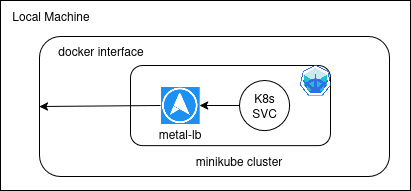
\includegraphics[width=0.8\textwidth]{Design/metal.png}
\end{figure}

From the figure, we can see that MetalLB is intended to be the frontend of our Kubernetes Cluster, ingesting data. It's important to note that MetalLB acts as a Layer 4 network load balancer, which allows it to proxy raw UDP packets into our cluster. This solves the problem of ingestion. The traffic will travel to and from the service, to MetalLB, and then to the outside cluster, and vice versa.



\subsubsection{Sequence Flow for metallb}
\begin{figure}[H]
\caption{Sequence flow for metal-lb}
\centering
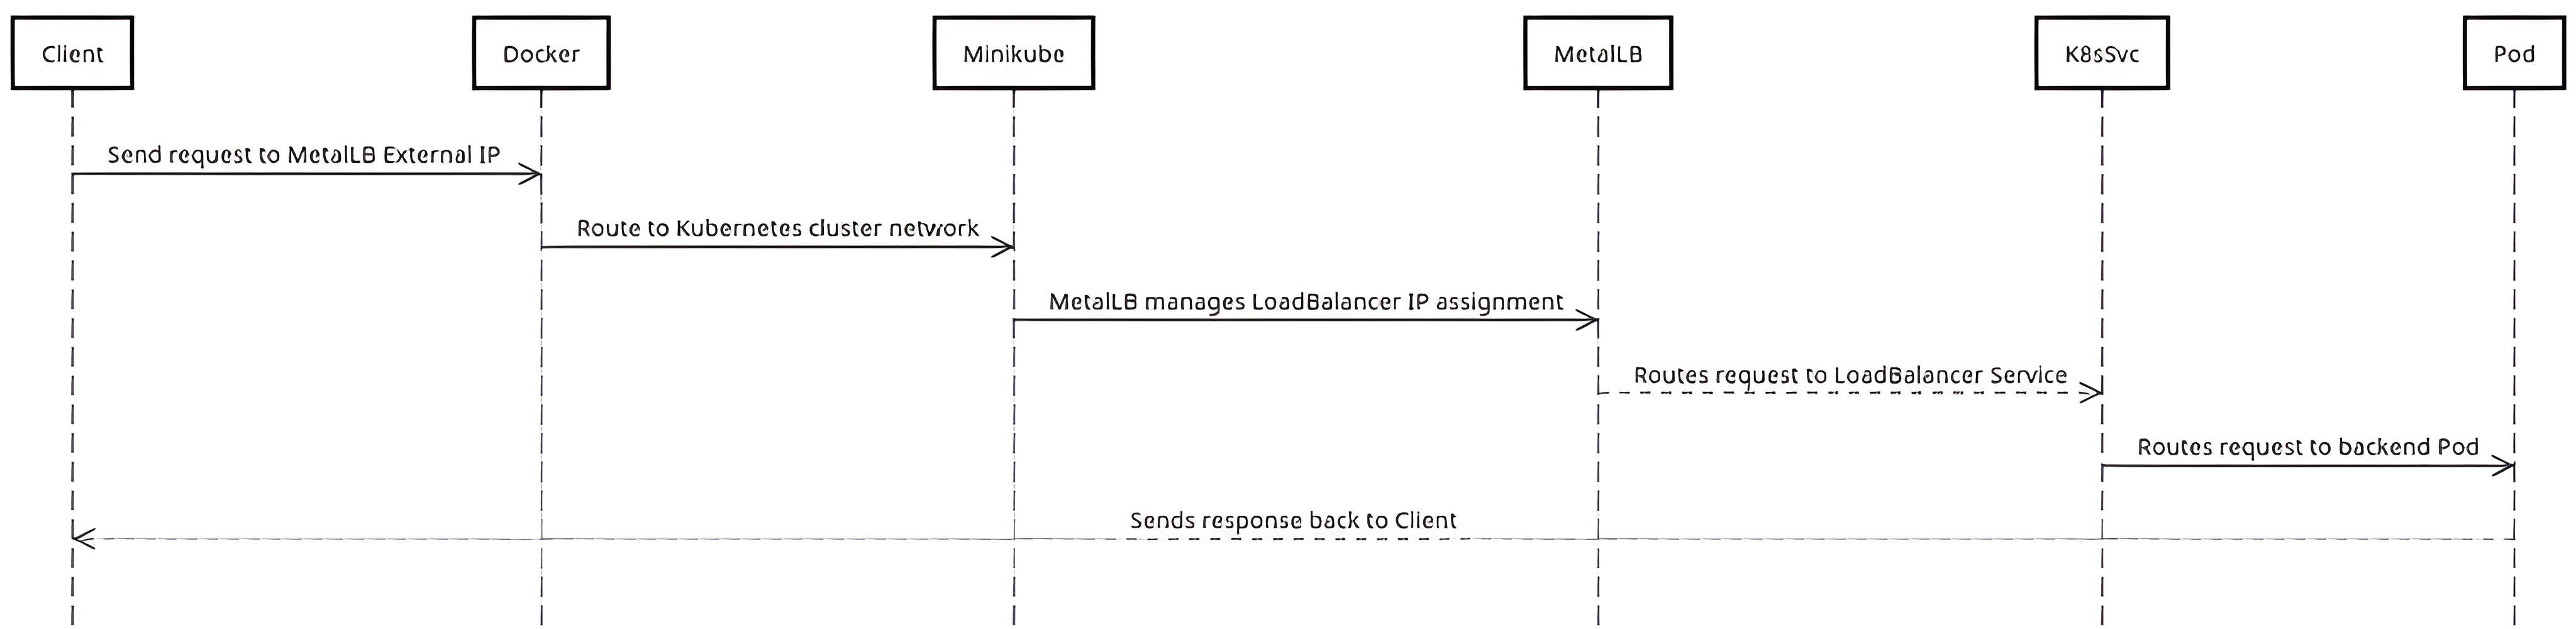
\includegraphics[width=1\textwidth]{Design/metal_sequence.png}
\end{figure}

The client sends a request to the MetalLB IP address. The request is then forwarded through the Docker interface, as MetalLB is deployed on the Minikube cluster, which is running in a Docker container. MetalLB receives the IP address and proceeds to forward the request to the Kubernetes service. This design successfully exposes the Kubernetes service to the outside cluster and allows for the forwarding of raw TCP and UDP packets to our applications.

\section{Design of the Routing and Processing System}

This section presents the design of the routing and processing system for a WebTransport stream-aware routing platform. Design focuses on optimization in configuration, connection managements, packets processing, use of metrics, integration of various microservices and flexibility in command line to facilitate a scalable and resilient streaming design.

\subsection{Configuration-Driven Routing Architecture}



The system adopts a configuration-driven routing approach that allows for dynamic changes and streamlined service management. A central `ServiceConfig` structure defines essential parameters—such as host, port, and endpoint—for each microservice, such as audio, video, chat. These configurations are written in a YAML file that is loaded during runtime using a dedicated `ConfigManager` component in Kubernetes. This component enables hot-reloading, so the routing logic can be changed without restarting services. The routing system can therefore be extremely flexible and extensible and easily reconfigured to accommodate emerging needs or varying deployment environments during operation of the system.

The architecture is intended to operate in Kubernetes and utilizes Kubernetes constructs such as ConfigMaps and Secrets to pass routing definitions and TLS credentials to the downstream code.As far as it is concerned, the Router Config is a central configuration file that encapsulates the rules of service routing and protocol behaviors. The router serves as a fast proxy, reading the configuration from this file and redirecting client search requests to the correct backend microservices. This decoupled and declarative model leads to routing behavior that is fully controlled entirely outside of the application's code. This approach aligns with CI/CD principles. The system supports dynamic scaling, safe updates, and operational agility, thereby enabling the router to be deployed in modern cloud-native operations that demand responsiveness and maintainability.


\begin{figure}[h]
\centering
\begin{tikzpicture}[
    box/.style={rectangle, draw, rounded corners, minimum height=2em, minimum width=6em, align=center},
    arrow/.style={-Stealth, thick}
]
    % Nodes
    \node[box] (yaml) at (0,0) {YAML Config};
    \node[box] (manager) at (4.5,0) {ConfigManager};
    \node[box] (service) at (9,0) {ServiceConfig};
    \node[box] (micro) at (13,0) {Microservices};

    % Arrows
    \draw[arrow] (yaml) -- (manager) node[midway, above] {Loads};
    \draw[arrow] (manager) -- (service) node[midway, above] {Parses};
    \draw[arrow] (service) -- (micro) node[midway, above] {Routes};
\end{tikzpicture}
\caption{Configuration-Driven Routing Flow}
\label{fig:config_routing}
\end{figure}

The figure illustrates the flow from a YAML configuration file to the \texttt{ConfigManager}, which parses and stores settings in \texttt{ServiceConfig} structures, enabling routing to microservices. Arrows indicate the sequential process of loading, parsing, and routing configuration data.

\subsection{WebTransport Protocol Handling}

The WebTransport protocol handling system manages QUIC/HTTP3 connections and streams, ensuring reliable communication for real-time streaming. A \texttt{WebTransportRouter} component handles protocol negotiation, stream creation, and HTTP/3 request processing, maintaining connection state. Each QUIC stream is assigned a dedicated buffer to manage packet reassembly and analysis, ensuring efficient handling of incoming data. This design supports high-throughput streaming while maintaining low latency and robust connection management.

\begin{figure}[h]
\centering
\begin{tikzpicture}[
    box/.style={rectangle, draw, rounded corners, minimum height=2em, minimum width=6em, align=center},
    arrow/.style={-Stealth, thick}
]
    % Nodes
    \node[box] (client) at (0,0) {Client};
    \node[box] (router) at (6.5,0) {WebTransportRouter};
    \node[box] (stream) at (13,0) {Stream Buffers};

    % Arrows
    \draw[arrow] (client) -- (router) node[midway, above] {HTTP3 Streams};
    \draw[arrow] (router) -- (stream) node[midway, above] {Assigns};
\end{tikzpicture}
\caption{WebTransport Protocol Handling}
\label{fig:webtransport}
\end{figure}

The figure depicts a client sending data via QUIC/HTTP3 to the \texttt{WebTransportRouter}, which assigns streams to dedicated buffers for processing. Arrows show the flow of data from the client to the router and then to stream buffers.

\subsection{Packet Parsing and Routing}

The packet parsing and routing system is designed to efficiently process incoming packets by extracting headers and forwarding payloads to the correct microservices. A fixed 32-byte header enables fast and reliable parsing, containing fields like \texttt{track\_id}, \texttt{payload\_len}, and \texttt{track\_type}. The payload is extracted based on the \texttt{payload\_len} field and routed to the appropriate microservice using the \texttt{track\_type} and configuration data. This design ensures low-latency processing and accurate routing in a multiplexed streaming environment.

\begin{figure}[h]
\centering
\begin{tikzpicture}[
    box/.style={rectangle, draw, rounded corners, minimum height=1.5em, minimum width=4em, align=center},
    arrow/.style={-Stealth, thick}
]
    % Nodes using absolute positioning
    \node[box] (packet) at (0,0) {Incoming Packet};
    \node[box] (parser) at (6,0) {Packet Parser};
    \node[box] (micro) at (12,0) {Microservices};

    % Arrows
    \draw[arrow] (packet) -- (parser) node[midway, above] {Parses};
    \draw[arrow] (parser) -- (micro) node[midway, above] {Routes};
\end{tikzpicture}
\caption{Packet Parsing and Routing}
\label{fig:packet_parsing}
\end{figure}

The figure shows an incoming packet being processed by the packet parser, which extracts the header and routes the payload to microservices. Arrows indicate the parsing and routing steps.


\subsection{Metrics Logging}
The structure of metrics logging is clearly elaborated in the evaluation (chapter 6). This part contains the overview of the design 


\begin{figure}[h]
\centering
\begin{tikzpicture}[
    box/.style={rectangle, draw, rounded corners, minimum height=1.5em, minimum width=4em, align=center},
    arrow/.style={-Stealth, thick}
]
    % Nodes
    \node[box] (client) at (0,0) {Client};
    \node[box] (router) at (6,0) {Router};
    \node[box] (logger) at (12,0) {Log to CSV};

    % Arrows
    \draw[arrow] (client) -- (router) node[midway, above] {Sends};
    \draw[arrow] (router) -- (logger) node[midway, above] {Logs};
\end{tikzpicture}
\caption{Client Request Routing and Logging}
\label{fig:client_logging}
\end{figure}


The figure illustrates the system collecting metrics via the \texttt{MetricsLogger}, which logs data to CSV and log files. Arrows represent the flow of metric collection and logging.

\subsection{Microservice Proxying}

The microservice proxying system forwards packets to the appropriate microservices with robust error handling and retry mechanisms. It supports flexible data formats, including binary and JSON, to accommodate different service requirements. Custom headers can be added to packets for extensibility and debugging, enabling traceability and future enhancements. This design ensures reliable communication between the router and microservices, supporting a modular and scalable architecture.



\begin{figure}[h]
\centering
\begin{tikzpicture}[
    box/.style={rectangle, draw, rounded corners, minimum height=1.5em, minimum width=4em, align=center},
    arrow/.style={-Stealth, thick}
]
    \node[box] (router) at (0,0) {Router};
    \node[box] (proxy) at (6,0) {Proxy Layer};
    \node[box] (micro) at (12,0) {Microservices};

    \draw[arrow] (router) -- (proxy) node[midway, above] {Forwards};
    \draw[arrow] (proxy) -- (micro) node[midway, above] {Routes};
\end{tikzpicture}
\caption{Microservice Proxying}
\label{fig:proxying}
\end{figure}

The figure shows the router forwarding packets to a proxy layer, which routes them to microservices with error handling. Arrows depict the forwarding and routing process.



\section{Pulsar Integration Design}

After processing packets such as chat messages, audio streams, or video data, each microservice can optionally publish the output to an Apache Pulsar topic. This mechanism decouples real-time data processing from downstream distribution analytics, storage, or machine learning. The messages of each particular service are sent to a specifically-named topic, such as chat-topic, video-topic, which guarantees a separation of concerns as well as scalability.

This design enables easy integration with real-time data consumers, allows for per-service configuration of Pulsar usage and allows for flexibility in order to enable/disable publishing dynamically.



\begin{figure}[h]
\centering
\begin{tikzpicture}[
    box/.style={rectangle, draw, rounded corners, minimum height=2em, minimum width=6em, align=center},
    arrow/.style={-Stealth, thick},
    topic/.style={rectangle, draw, minimum height=2em, minimum width=6em, align=center}
]

% Nodes
\node[box] (micro) at (0,0) {Microservice};
\node[box] (producer) at (4,0) {Pulsar Producer};

% Topic nodes
\node[topic] (chat) at (8,2) {chat-topic};
\node[topic] (video) at (8,0.5) {video-topic};
\node[topic] (audio) at (8,-1) {audio-topic};

% Arrows
\draw[arrow] (micro) -- (producer);
\draw[arrow] (producer) -- (chat);
\draw[arrow] (producer) -- (video);
\draw[arrow] (producer) -- (audio);

\end{tikzpicture}
\caption{Microservice to Pulsar Topics Integration}
\label{fig:microservice_pulsar}
\end{figure}



\section{Complete System Architecture}

The following architecture is a high-level technical architecture diagram which entails the complete proposed solution. The sections above delved deep into each components individually and this is the final high-level overview of our dissertation

\begin{figure}[H]
\caption{System Architecture}
\centering
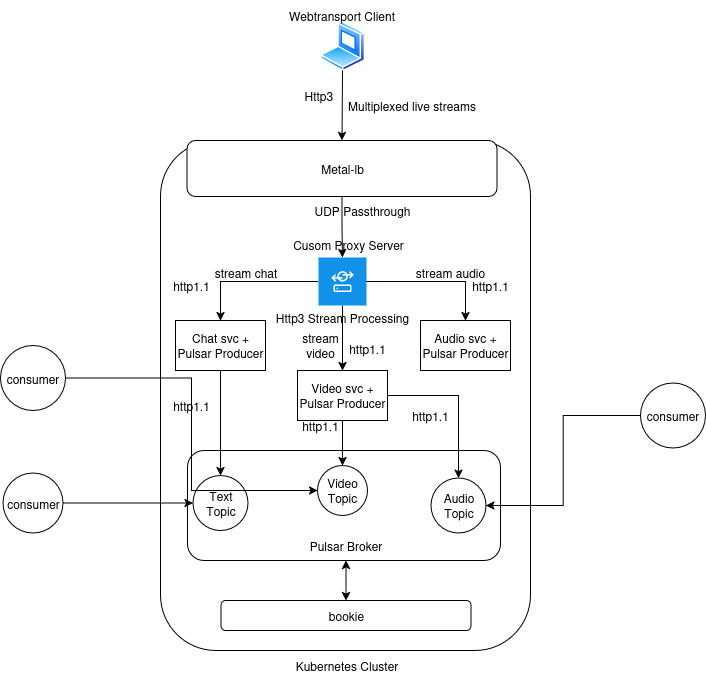
\includegraphics[width=1\textwidth]{Design/Design_Solution.png}
\end{figure}

The proposed architecture system is a real-time streaming system based on a modular structure built to support scaling, low latency communication, and efficient data processing and distribution within a cloud-native infrastructure. It starts with ingest layer where client sends streams of data with a webtransport client connects through HTTP/3 a QUIC-based protocol allowing to establish a single transport connection but with multiplexing multiple data streams in the connection video, audio, and chat. The load balancer in the Kubernetes cluster is MetalLB, which is exclusively enabled to provide UDP passthrough for the minikube ckuster to facilitate the forwarding of QUIC connection (entire UDP packets) to the internal components. The system is centered around a custom proxy server that will terminate the HTTP/3 connection, demultiplexes the stream it receives, and forwards each individual data stream to the appropriate microservice over HTTP/1.1. This server effectively acts as both a protocol gateway and a routing mechanism.

The application layer is based on different microservices of chat, video, and audio developed which is responsible for handling its own set of data and are independent from each other. These microservices publishes the data to Apache Pulsar after processing, acting as a producer in the event streaming system. The Pulsar cluster will have a broker handling the routing and dispatching of messages, different topics that logically segregate each type of data (Text Topic, Video Topic, Audio Topic) and it will have a persistent storage backend consisting of the Bookie pods of Apache BookKeeper so that persistant data storage and recovery from faults are possible. Finally, on the consumption level, independent consumer applications subscribes to the Pulsar topics and receive data asynchronously. This decouples the data ingestion and downstream processing, allowing to enable use cases of real-time streaming, analytics or storage with modularity and scalability in the system.
\label{sec:OverviewOfDesign}

\section {Summary}
The proposed system is a real-time streaming architecture that is modular and scalable, designed to support low-latency multimedia communication using WebTransport, Kubernetes, and Apache Pulsar. The architecture breaks the problem space into smaller modules which are developed independently and then combined to form a whole solution. On the client side, WebTransport is used to send data, and WebTransport runs on QUIC to enable data multiplexing across different data streams in a single connection i.e. audio, video and chat. The design will prevent Head-of-Line blocking. A typical packet transmitted has a 32-byte header composed of track\_id, payload\_len and track\_type fields and a variable length payload. The format is capable of extending; it is useful in routing for diversity of data types.

Inside the Kubernetes cluster, a single-node Minikube setup is used for simplicity, leveraging the Docker driver to eliminate virtual machine overhead and enable shared networking. MetalLB is used as a bare metal load balancer that exposes QUIC-based UDP traffic to components of the kubernetes cluster, enabling the external WebTransport clients to connect to internal services. Its routing logic is config-driven, user-managed through YAML-based ConfigMaps and allows for dynamic updates and reloading of routing configurations without system restarts. The core of this solution is the WebTransportRouter, a custom component that accepts and deals with QUIC/HTTP3 streams by attaching each track with its own explicitly associated buffer of streams. This guarantees that audio, video and chat information is manipulated in a low latency basis for redirections. Once the component performs initial parsing, it sends each stream to its respective microservice through HTTP/1.1 via a proxy server that acts as a reliable gateway between the transport and application layers.

At the application layer, separate stateless microservices are responsible for processing specific types of data such as audio, video, or chat. Each microservice publishes the processed data to its corresponding Apache Pulsar topic—for instance, chat-topic or video-topic—thereby enabling a decoupled and scalable processing model. Apache Pulsar is used as the main system for handling event streams. It consists of a broker which receives data for a specific topic and it stored multiple topic's logical association, with each topic keeping different types of data separate (like audio, video, or chat). To ensure data is safely stored and can be recovered if something goes wrong, Apache BookKeeper is used in the background through components called Bookie. On the receiving side, different consumer applications connect to Pulsar and subscribe to specific topics to get the data they need. By keeping the parts that send, process, and receive data separate, the system stays flexible, reliable, and easy to scale for real-time streaming or analytics tasks.


% \section{Detail 1 of the Design}
% \subsection{Aspect \#1}

% \subsubsection{Detail of Aspect  \#1}

% \subsubsection{Another Detail of Aspect  \#1}


% \subsection{Aspect \#2}

% \subsubsection{Detail of Aspect  \#2}

% \subsubsection{Another Detail of Aspect  \#2}


% \section{Detail 2 of the Design}

% \section{Summary}
% \label{sec:SummaryDesign}

% Every chapter aside from the first and last chapter should conclude with a summary. 